\chapter{Ergebnisse}

\section{Evaluation der Anwendung}\label{Evaluation der Anwendung}
Alle funktionalen Anforderungen sind im Prototyp der Anwendung in Javascript mit dem node.js-Framework und dem socket.io-Websocket (Abschnitt \ref{socket.io-Server} und \ref{socket.io-Client}) vollständig umgesetzt. Im Screenshot des Hamburger Hafens (Abb. \ref{Hafen Hamburg}) kann man erkennen, dass liegende Schiffe als Kreise dargestellt werden und fahrende Schiffe als Richtungsdreiecke. Wurden Masse übermittelt (AIS-Nachricht vom Typ 4), sind maßstabsgetreue Polygone eingezeichnet, deren Farbe den Schiffstyp kennzeichnet.
Ein Popup mit Detailinformationen zum dem Schiff links daneben ist geöffnet. In dieser Zoomstufe ist die Animation bereits aktiv, das heißt für den Betrachter, dass alle angezeigten Richtungsdreiecke ununterbrochen in Bewegung sind.

\begin {figure}[H]
\begin{center}
  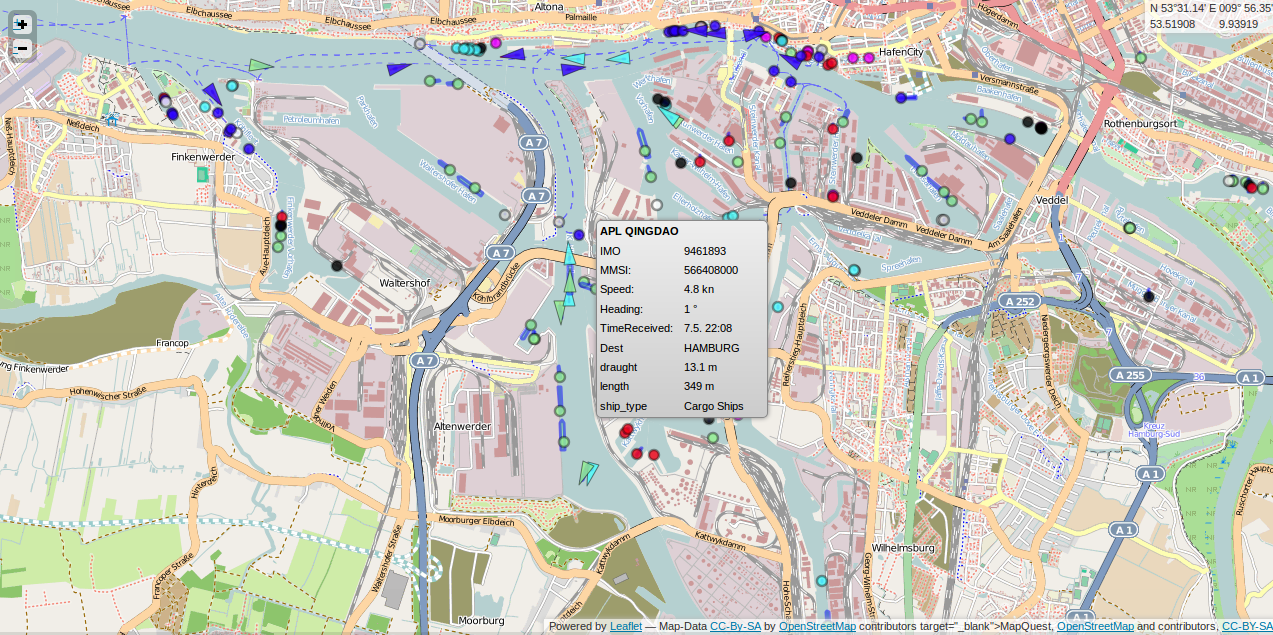
\includegraphics[width=6in]{images/Hamburg.png}
\end{center}
\caption{Anzeige aller Schiffe im Hamburger Hafen}
\label{Hafen Hamburg}
\end {figure}
Das zweite Beispiel zeigt die Situation bei niedriger Zoomstufe (Abb. \ref{Nordsee}). Oben links in der Karte ist ein Hinweis eingeblendet, dass nur Schiffe mit einer Geschwindigkeit über 12 Knoten angezeigt werden. Die Verteilung des Schiffsverkehrs lässt sich gut erkennen, während die große Zahl hafenliegender Schiffe ausgespart bleibt, um die Performance des Browser-Clients zu erhalten. Aus demselben Grund ist die Animation ausgeschaltet. Durch die große Anzahl empfangener Positionsmeldungen, ist die Darstellung trotzdem bewegt.

\begin {figure}[H]
\begin{center}
  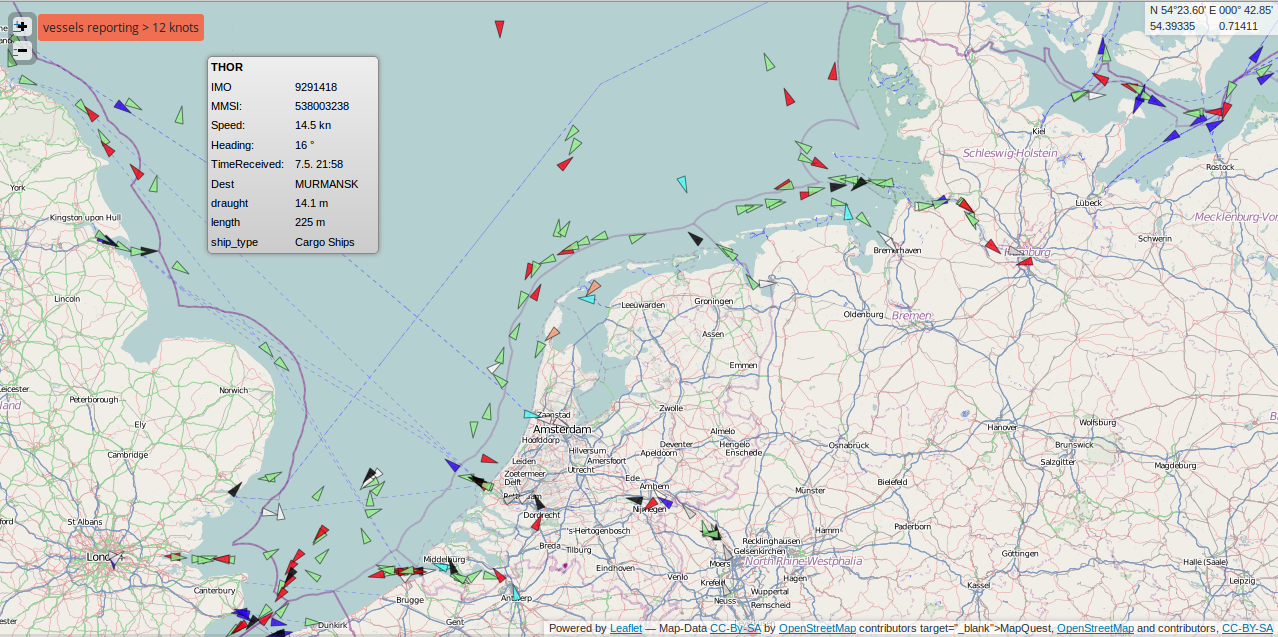
\includegraphics[width=6in]{images/zoomout.png}
\end{center}
\caption{Auf schnell fahrende Schiffe reduzierte Anzeige am Beispiel der Nordsee}
\label{Nordsee}
\end {figure}

\begin {wrapfigure}[9]{r}{3in}
\begin{center}
  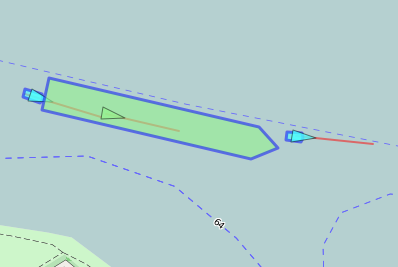
\includegraphics[width=2in]{images/Schleppen.png}
 \caption{Schleppmanöver}
  \end{center}
 \label{Schleppmanöver}

\end {wrapfigure}


Schließlich ist in hohen Zoomstufen eine Beobachtung von aktuellen Schiffsmanövern möglich, wie im Beispiel \ref{Schleppmanöver} das Schleppen eines Frachtschiffes durch zwei Schleppschiffe. Durch die hohe Frequenz der Positions-Meldungen bei fahrenden Schiffe und mithilfe der eingebauten Animation erlebt der Betrachter die Szene wie in einem Animationsfilm.\\

Mit dieser Implementierung wurde auch die wichtige nicht funktionale Anforderung nach einer zeitnahen Umsetzung erfüllt. Der Prototyp wird auf github als privates Repository gehostet und konnte nach der Übergabe (Ende Januar) vom Unternehmen vesseltracker für Weiterentwicklungen der Webanwendung und Kundenprojekte verwendet werden. 
Desweiteren ist die gesamte Anwendung mit open source Produkten entwickelt worden und verwendet das von vom Unternehmen gehostete Kartenmaterial.\newline
Die Anwendung wurde auf den unten angegebenen Browserclients in den angegebenen Versionen positiv auf Funktionalität getestet und unterstützt damit die gängisten Browser in den einschlägigen Versionen \footnote{http://www.browser-statistik.de/statistiken/versionen/}:
\begin{itemize}
\item Firefox Version 15.0.1 und 20.0
\item Google Chrome 26.0
\item Internet Explorer Version 9.0 und 10.0, und Version 7 und 8 im Kompatibilitätsmodus von IE 10
\item Safari 6.0.4
\end {itemize}

Die Latenzzeit zwischen dem Empfang der AIS-Positions-Meldung durch den Rohdatenserver und der Propagierung derselben Position auf der Karte sollte unterhalb 500 msec liegen. 
\begin {wraptable}{r}{3in}
\begin{center}
\begin{tabular}{| l|r|}\hline
& [msec]\\\hline
Mittelwert & 237 \\
Maximum & 701\\
Minimum & 23\\\hline
\end{tabular}
\caption[Latenzzeit von Positionsmeldungen in der RealtimeAnwendung]{Latenzzeit von Positionsmeldungen in der Realtime-Anwendung}
\label{Latenzeit_RealtimeApp}
\end{center}
 \end {wraptable}
Untersucht wurde die Latenzzeit anhand der ‘time\_received’, die vom Rohdatenserver jeder AIS-Message als Zeitstempel beim Empfang hinzugefügt wird. Auf dem Rohdatenserver läuft ein ntp-Daemon zur Zeitsynchronisation. Ebenso ein Daemon wurde auf dem Client, auf dem der Browser läuft gestartet und ein Zeitstempel genommen, nachdem das Schiff mit der neuen Position auf die Karte gerendert wurde. Weil die Latenzzeit direkt abhängig ist von der Anzahl der Meldungen, die pro Zeit vom Client emfangen werden, wurde als Referenz eine Ansicht des Hamburger Hafens gewählt in Zoomstufe 12, der niedrigsten Zoomstufe, in der noch Schiffe jeder Geschwindigkeit angezeigt werden. Die Ergebnisse (Tabelle \ref{Latenzzeit}) liegen mit dem Mittelwert gut innerhalb der geforderten Geschwindigkeit.

Die Anzahl der Verbindungen, die der Server gleichzeitig bedienen kann, ist mit einem node.js-Script getestet worden, das alle 500 ms eine neue Clientverbindung erstellt, bis 750 Clients verbunden sind. Der Aufbau der Verbindung geschah auch mit steigender Verbindungsanzahl zuverlässig, jedoch ist in der Abbildung erkennbar, dass die Anzahl der Fälle zunimmt, in denen ein Client lange auf Antwort warten muss.
\\Eine Skalierung der Serveranwendung ist seitens des socket.io-Servers kein Problem. Statt einen einzigen Worker-Prozess zu generieren, können auch mehrere Worker-Prozesse parallel gestartet werden, die alle dieselbe mongo-Datenbank-Collection abfragen und sich bei derselben redis-Datenbank im Channel ‘positionUpdate’ registrieren können. Allerdings muss sichergestellt sein, z.B.  über unterschiedliche Ports oder unterschiedliche (virtuelle) Server, dass ein verbundener Client mit jedem neuen Request auf demselben Worker-Prozess landet.

\begin{figure}[H]
\begin{minipage}[hbt]{3in}
	\centering
	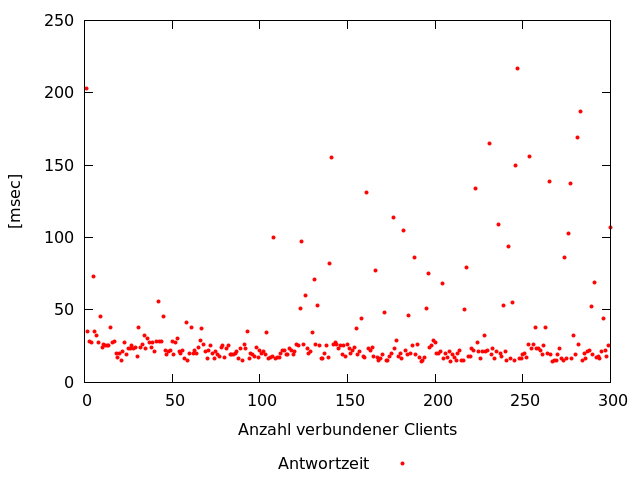
\includegraphics[width=2.5in]{images/stresstest300.png}
	\label{Stresstest300}
\end{minipage}
\hfill
\begin{minipage}[hbt]{3in}
	\centering
	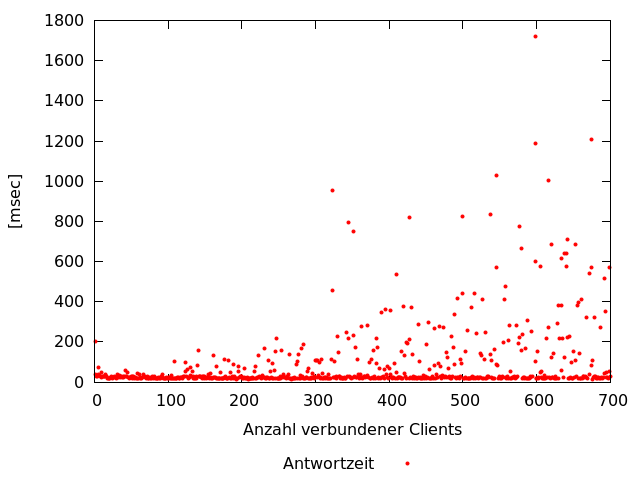
\includegraphics[width=2.5in]{images/stresstest.png}
	\label{Stresstest}
\end{minipage}
\caption{Anwortzeiten des socket.io-Websocket-Servers in Abhängigkeit von der Anzahl verbundener Clients}
\end{figure}
%-------------------------------------------------------------------------------------------------------------------------------------------
\section{Vergleichende Evaluation der Javascript- und der Dart-Anwendung}
Die in Google Dart geschriebene Client-Anwendung soll nun mit dem in Javascript programmierten Client verglichen werden. Die in den Abschnitten  \ref{Strategie-Korrektur} und \ref{Vergleichbarkeit} begründete zusätzliche Implementierung eines HTML5-kompatiblen node.js-Websocket-Servers muss nun in einem ersten Schritt mit dem node.js-socket.io-Server verglichen werden. Für diesen und alle folgenden Tests wurde auf dem Rohdatenserver ein Port eingerichtet, der nur die Daten von drei AIS-Antennen (Hamburg, Wedel, Geesthacht) ausgibt. Dies war notwendig, um den als Server verwendeten Arbeitsplatzrechner (MHz und 1 GB Arbeitsspeicher) nicht zu überlasten. Dadurch entstünde eine zusätzliche Latenzzeit wegen des kontinuierlichen Anwachsens der Messagequeues auf dem Server, die die Ergebnisse verzerrt.
%-------------------------------------------------------------------------------------------------------------------------------------------
\subsection{Node.js - socket.io-Socket-Server vs. node.js-Websocket-Server}\label{socket.io- vs html5-Server}
\subsubsection{Implementierungsaufwand}
Im Implementierungsaufwand unterscheiden sich beide Server- und Client-Anwendungen kaum (Anzahl zeilen code).  Einige Features der socket.io-Bibliotheken (z.B. die Clientverwaltung, Parameter für ‘Production’ und ‘Development’-Umgebung bezüglich Log-Leveln, Client-Minifikation oder Client-Zip) sind praktisch und müssten in der Alternativimplementierung für den Einsatz in einer produktiven Umgebung anderweitig gelöst werden. Durch die in socket.io eingeführten Events vermindert sich der Kommunikationsaufwand zwischen Server und Client geringfügig, was in diesem Fall einer datenintensiven Anwendung mit großen Datenmengen pro Nachricht wenig zu Buche schlägt.
\subsection{Latenzzeit}
Die Leistungsfähigkeit beider Implementierungen wird verglichen, indem wieder wie in Tabelle \ref{Latenzeit_RealtimeApp} die Zeit gemessen wird, die eine Positionsmeldung braucht für den Weg vom Rohdatenserver bis zur Präsentation auf der Karte. Um eine ähnliche Situation in beiden Szenarien abzubilden, wurde jeweils eine bestimmte Position in Hafen Hamburg angesteuert und ein Timer in die Client-Anwendung integriert, der jeweils nach einer Minute um eine Stufe herauszoomt. Da ab Zoomlevel 11 und kleiner nur noch Schiffe mit einer jeweils definierten Mindestgeschwindigkeit angezeigt werden, nahm die Anzahl empfangener Schiffe von dieser Zoomstufe an wieder ab. Zur Auswertung wird auf dem Client ein LogFile geschrieben, das pro Nachricht, deren ‘time\_received’ und einen aktuellen Zeitstempel schreibt.  Die Differenz wird als Latenzzeit interpretiert. Anschließend wird über das Logfile berechnet, wieviele Positionsmeldungen in einer Minute an den Client gesendet wurden. Darüber ist es möglich, die Latenzzeit gegen die Anzahl empfangener Positionsmeldungen pro Minute darzustellen, wie in Abbildung \ref{Latenzzeit socket.io} und \ref{Latenzzeit HTML5} zu sehen.
\begin {figure}[H]
\begin{center}
  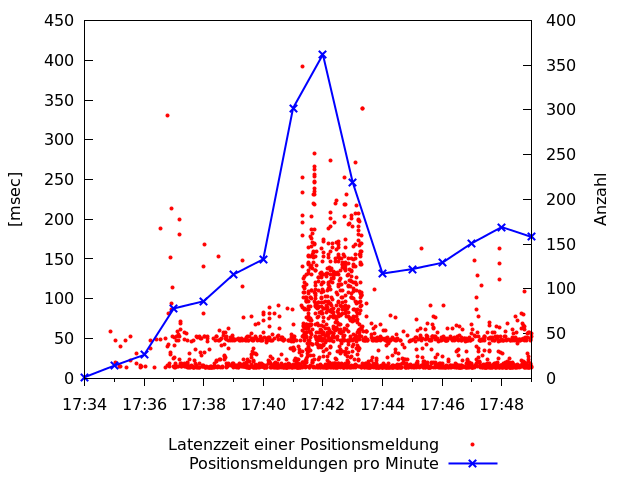
\includegraphics[width=4.5in]{images/latency_timeReceived_socket_io.png}
\end{center}
\caption{socket.io-Websocket-Server: Latenzzeit der Positionsmeldungen und Anzahl empfangener Schiffe}
\label {Latenzzeit socket.io}
\end {figure}

\begin {figure}[H]
\begin{center}
  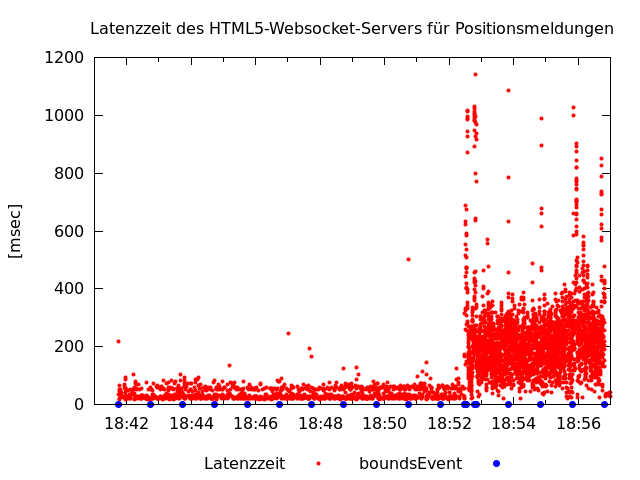
\includegraphics[width=4.5in]{images/latency_timeReceived_HTML5.png}
\end{center}
\caption{HTML5-Websocket-Server: Latenzzeit der Positionsmeldungen und Anzahl empfangener Schiffe}
\label {Latenzzeit HTML5}
\end {figure}
Es ist offensichtlich, dass die Geschwindigkeit in der Darstellung von der Anzahl empfangener Nachrichten linear abhängt.
Darüber hinaus ist zu erkennen, dass beide Implementierungen ihre Aufgabe in ähnlicher Geschwindigkeit erledigen. 

\subsection{Browserunterstützung}
Für die  node.js-HTML5-Websocket-Anwendung wird wie für die socket.io-Websocket-Anwendung in Abschnitt \ref{Evaluation der Anwendung} die Unterstützung durch die gängigsten Browser getestet. Die Ergebnisse sind in Tabelle \ref{Browserclients-Vergleich} gegenübergestellt.

\begin{table}
\begin{tabular}{ l|l|c|c}
Browser&Version&socket.io-Anw.&HTML5-Anw.\\\hline
Firefox& 20.0&websocket&websocket \\
Google Chrome & 26.0 &websocket&websocket\\
Internet Explorer&9& Fallback auf Flashsocket&nicht unterstützt\\
Internet Explorer&10& websocket&websocket\\
Safari&6.0.4 & websocket&websocket\\
\end{tabular}
\caption[Unterstützung von Browserclients im Vergleich socket.io vs. HTML5]{Unterstützung von Browserclients im Vergleich socket.io vs. HTML5}
\label{Browserclients-Vergleich}
\end{table}

\section{Javascript-Client vs. Dart-Client} 
\subsection{Implementierungsaufwand}
Beim Programmieren bietet Dart nach einer kurzen Einarbeitung einige Erleichterungen gegenüber der Javascript-Programmierung. Besonders ist das objektorientierte Programmieren in Dart sehr viel intuitiver möglich als in Javascript, wie leicht in Abbildung \ref{} zu erkennen. Javascript bietet zwar zahlreiche Lösungen, um Objektorientiertheit herzustellen über Funktionen als Objekte oder Konstrukte wie das Revealing Module Pattern, das aber verlangt javascript-spezifisches Hintergrundwissen und schafft keine vergleichbare Struktur.
Die Dart-Implementierung der Anwendung wird an dem Punkt etwas aufwendiger, wo über das Paket js-interop die Javascript-Dateien integriert werden und Proxies und Callback-Funktionen geschrieben werden müssen zur Kommunikation zwischen dem Javascript- und dem Dart-Namensraum.
Mit dem dart2js-Compiler ließ sich der Dart-Client-Code zu Javascript kompilieren und war dann auch auf Browsern ohne Dart VM ausführbar.
\subsection{Performance}
Um die unterschiedliche Performance des Javascript-Client, des eigentlichen Dart-Clients und des zu Javascript kompilierten Dart-Clients zu vergleichen, wurde der VesselInBounds-Event genutzt. Gemessen wurde die Zeit, die benötigt wird, um nach Empfang eines VesselInBounds-Events alle in der Message enthaltenen Schiffe auf die Karte zu rendern. Verglichen wurden die Clients in den Browsern Dartium, Chrome und Firefox.
\begin{itemize}
\item Google Dartium interpretiert den originären Dart-Client mit der Dart VM. Beim Aufruf des Javascript-Clients wird der Javascript-Code mit der V8-Javascript-Engine interpretiert.
\item Google Chrome  mit der V8-Javascript-Engine führt beim Aufruf des Dart-Clients den zu javascript kompilierten Dart-Code aus und beim Aufruf des Javascript-Clients den originären Javascript-Code.
\item ebenso führt Firefox mit der SpiderMonkey Javascript Engine den zu Javascript kompilierten Dart-Client-Code, bzw. den originären Javascript-Client-Code aus.
\end {itemize}


\begin {figure}[H]
\begin{center}
  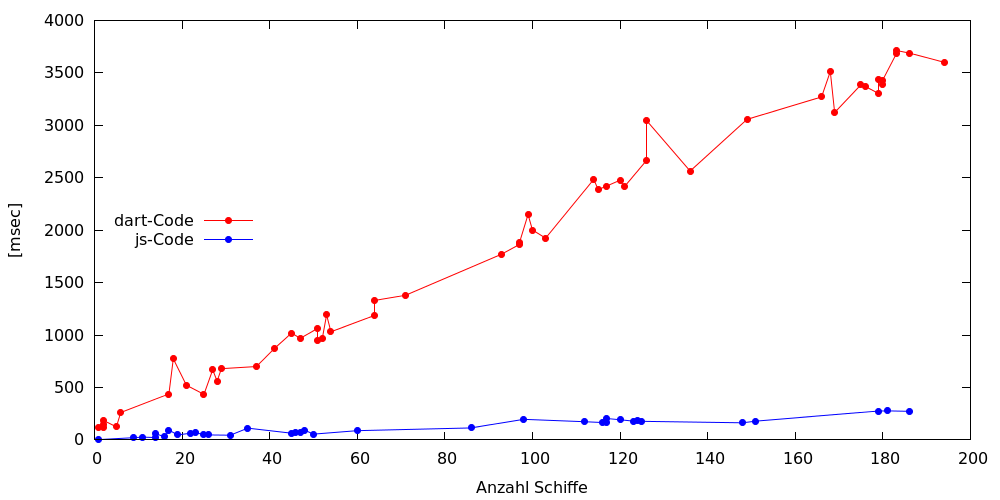
\includegraphics[height=2.3in]{images/Dartium.png}
\end{center}
 \caption{Dauer des Renders in Dartium}
\end {figure}


\begin {figure}[H]
\begin{center}
  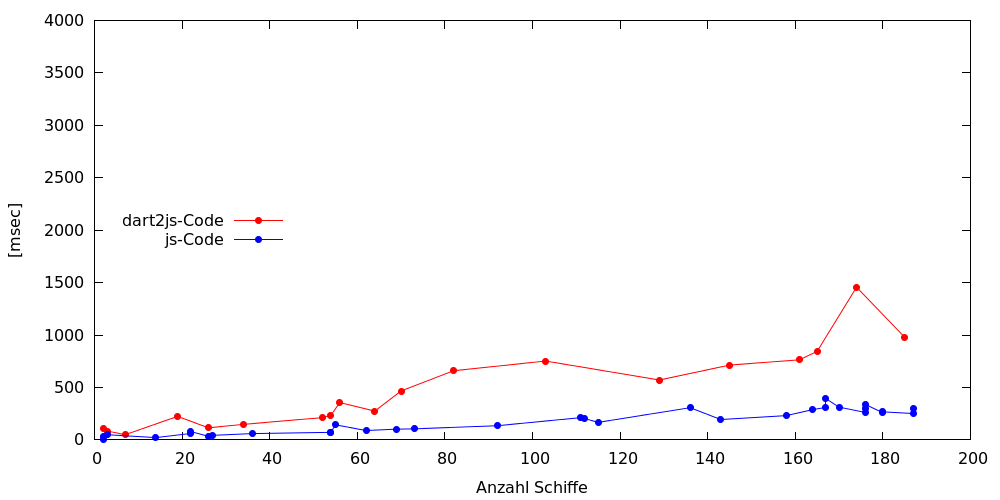
\includegraphics[height=2.3in]{images/Chrome.png}
\end{center}
 \caption{Dauer des Renders in Chrome}
\end {figure}


\begin {figure}[H]
\begin{center}
  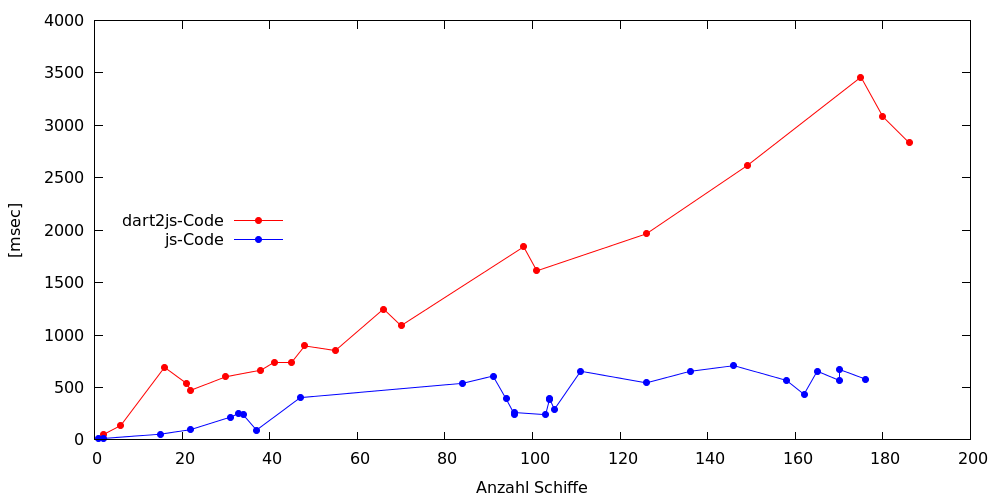
\includegraphics[height=2.3in]{images/Firefox.png}
\end{center}
 \caption{Dauer des Renders in Firefox}
\end {figure}

Insgesamt ist erkennbar, dass der Javascript-Code schneller ausgeführt wird als der Dart-Code. Am schnellsten führt die V8-Javascript-Engine in Dartium und Chrome den originären Javascript-Code aus. Firefox mit der Spidermonkey-Javascript-Engine benötigt deutlich länger. Auffällig ist, dass der Dart-Code von der Dart VM in Dartium langsamer ausgeführt wird als der zu Javascript kompilierte Code in Chrome. 



\subsection{Browserunterstützung}
\subsubsection{Dartium}

\subsubsection{Firefox, Chrome, IE, Safari}

Der dart-Client kompiliert den in Dart geschriebenen Code zu Javascript.

Dabei traten Fehler auf, die unter Dartium (also im originalen Dart-Code) nicht auftraten.
1. Wird innerhalb des Javascript-Scopes eine Methode auf einen javascript-Proxy (hier \_map) aufgerufen und ein proxy wird zurückgegeben, dann ist es nicht möglich auf diesen Proxy, der in diesem Fall vom Typ LatLngBounds sein müsste, eine Methode der Klasse LatLngBounds aufzurufen. => TypeError: t1.get\$\_map(...).getBounds\$0(...).getSouthWest\$0 is not a function

dart-client: web/leaflet\_maps.dart

  List getBounds(){
    var south, west, north, east;
    js.scoped((){
    south= \_map.getBounds().getSouthWest().lng;
        west = \_map.getBounds().getSouthWest().lat;
        north = \_map.getBounds().getNorthEast().lng;
        east = \_map.getBounds().getNorthEast().lat;
 });
return [west, south, east, north];
    
In diesem Fall wird einfach als work-Around eine andere Methode verwendet (getBBoxString), die einen String mit den Bounds zurückgibt. Aus den Teilen dieses Strings werden mit der Methode parse(string) der Klasse double die Werte der Eckpunkte der Bounds generiert.

String getBounds(){
    String bBox;
    js.scoped((){
      bBox = \_map.getBounds().toBBoxString();
    });
    return bBox;
  }

 Weil dadurch der message-Parameter 'bounds' kein number-Array, sondern ein String ist, muss im html5-Server der String einmal zum Float geparst werden.



2. Ein Feld ("IMO") wird auf null und auf > 0 geprüft.


\chapter{Fazit}\label{Fazit}
 \section{Ergebnisse }
\subsection{Die Realtime-Applikation}


Features, die in die Anwendung integriert werden sollten:
\begin{itemize}
\item eine aufklappbare Liste, in die der Nutzer favorisierte Häfen speichern kann, die dann mit einem Klick angesteuert werden können.
\item eine Legende mit einer Erläuterung der farbigen Schiffssymbole
\item zur weiteren Optimierung der Anwendung, sollte die Möglichkeit, die Animation der Richtungsdreiecke und Schiffspolygon über css3-Transition-Funktionen zu realisieren, unbedingt weiterverfolgt werden
\end{itemize}

\subsection{Vergleich Javascript und Google Dart}

Wie in den Abbildung zur Struktur der Anwendung erkennbar, ist mit Dart sehr viel einfacher Objektorientiertheit herzustellen. Dadurch wird die Anwendung einfacher zu verstehen und entsprechend einfacher zu entwerfen, zu schreiben und zu warten.
Das Erlernen von Dart ist für Umsteiger von Javascript relativ einfach möglich. Von den vielen Features und Möglichkeiten, die Dart bietet, kommt in der Client-Anwendung zwar nur ein kleiner Teil zum Tragen. Das Ziel war hier nicht das Ausschöpfen der Möglichkeiten von Google Dart, sondern die Realisierung eines kleinen Projektes alternativ in Google Dart.
Sehr hilfreich war der DartEditor als Entwicklungsumgebung, dessen Compiler bei Syntax-Fehlern aussagekräftige Warnungen ausgibt. 
Google Dart befindet sich noch in der Entwicklungsphase, so dass gelegentlich nach den ca. wöchentlichen Versions-Updates von Dart die Anwendung unter der neuen Version nicht mehr lauffähig ist und angepasst werden muss. Belohnt wird der Aufwand sozusagen mit einer kontinuierlichen Verbesserung der Performance im Laufe des letzten halben Jahres.
Das Einbinden existierender Javascript-Bibliotheken mit js-interop erweitert die Nutzungsmöglichen von Dart ganz entscheidend. Das Arbeiten mit zwei unterschiedlichen Scopes (Javascript und Dart) ist aber am Anfang sehr fehleranfällig. Und die Fehler sind schwierig zu debuggen, weil die Debugger (hier Firebug und der Debugger im DartEditor) nicht über die Grenzen des Namensraumes wechseln können.

\section{Ausblick}
Legende
-Satellitendaten in die Anwendung einbinden
%http://en.wikipedia.org/wiki/Comparison_of_layout_engines_%28ECMAScript%29#ECMAScript_version_support
